\section{Analyzer::Base2D Class Reference}
\label{classAnalyzer_1_1Base2D}\index{Analyzer::Base2D@{Analyzer::Base2D}}
{\tt \#include $<$analyzerbase.h$>$}

Inheritance diagram for Analyzer::Base2D:\begin{figure}[H]
\begin{center}
\leavevmode
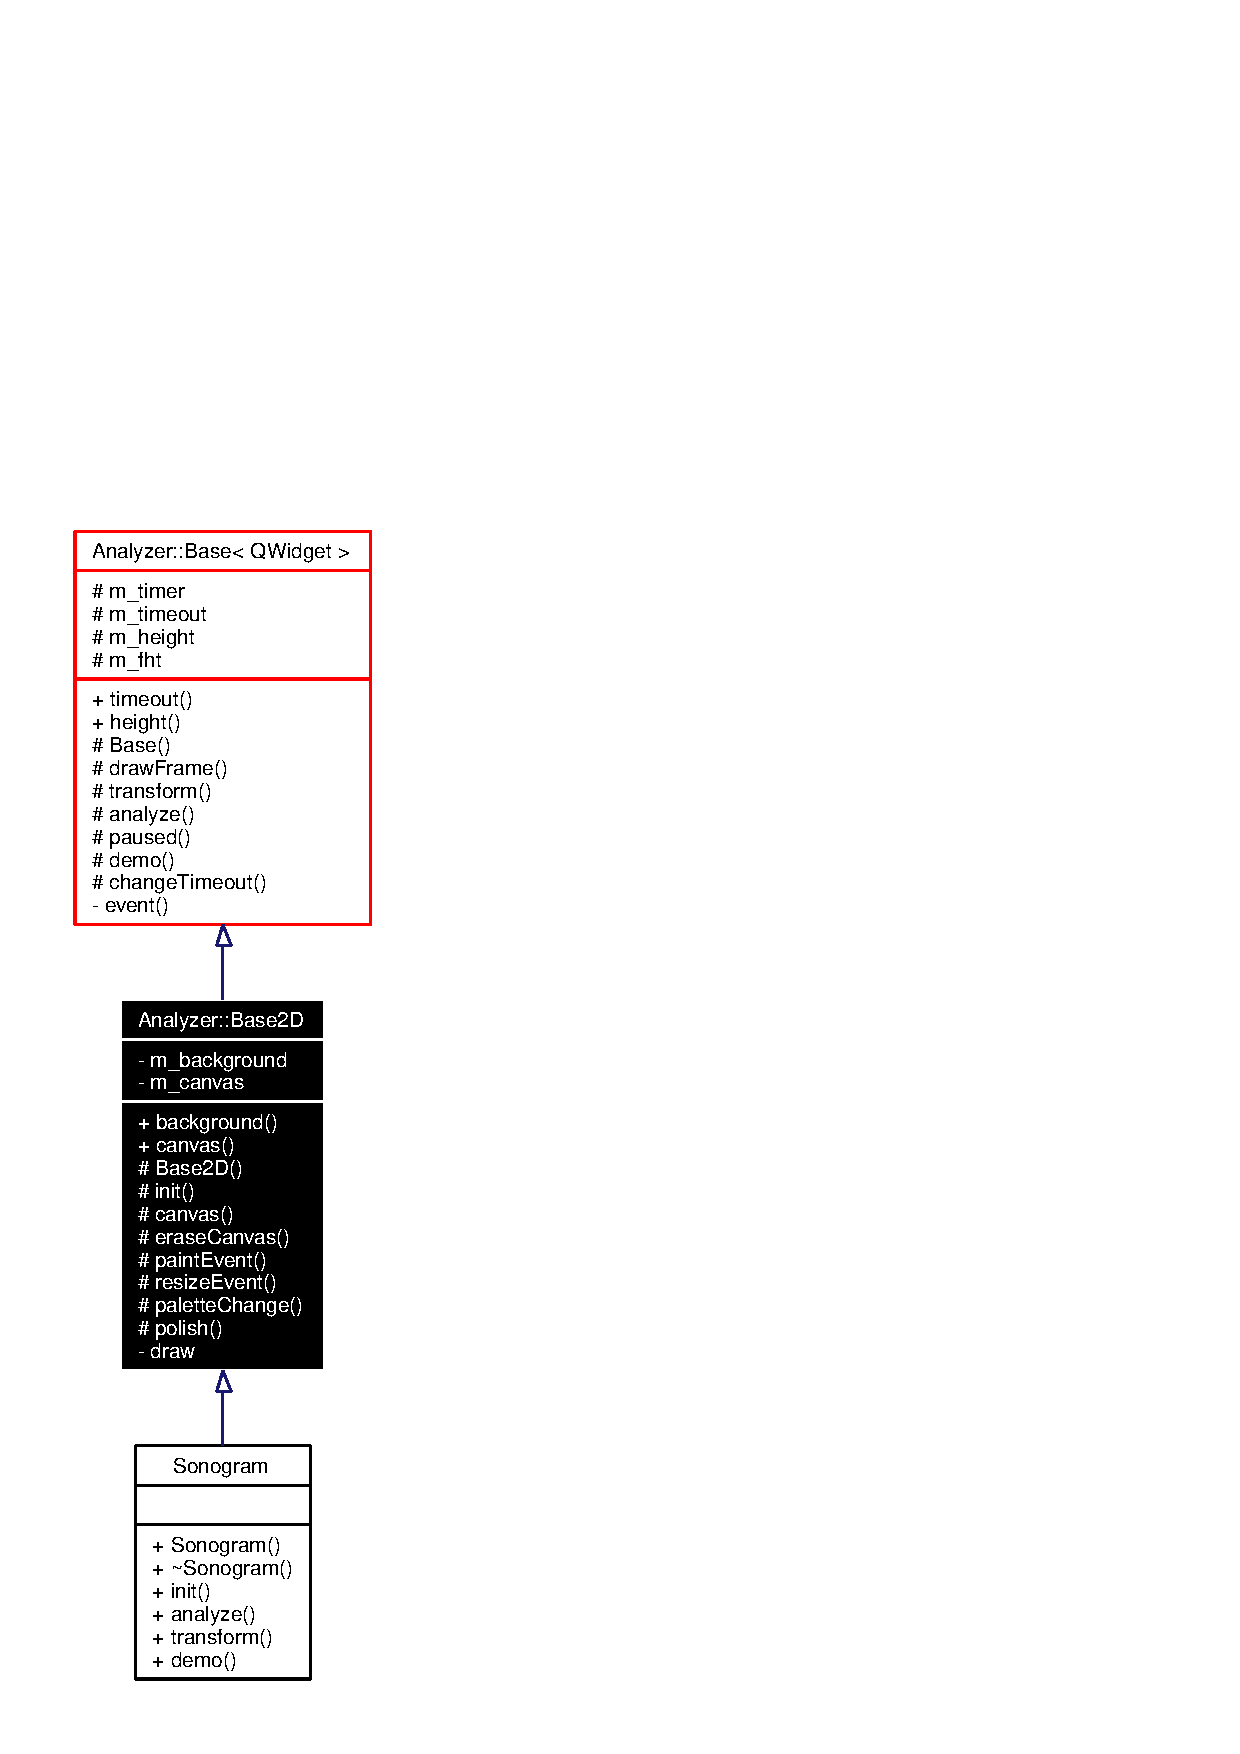
\includegraphics[width=89pt]{classAnalyzer_1_1Base2D__inherit__graph}
\end{center}
\end{figure}
Collaboration diagram for Analyzer::Base2D:\begin{figure}[H]
\begin{center}
\leavevmode
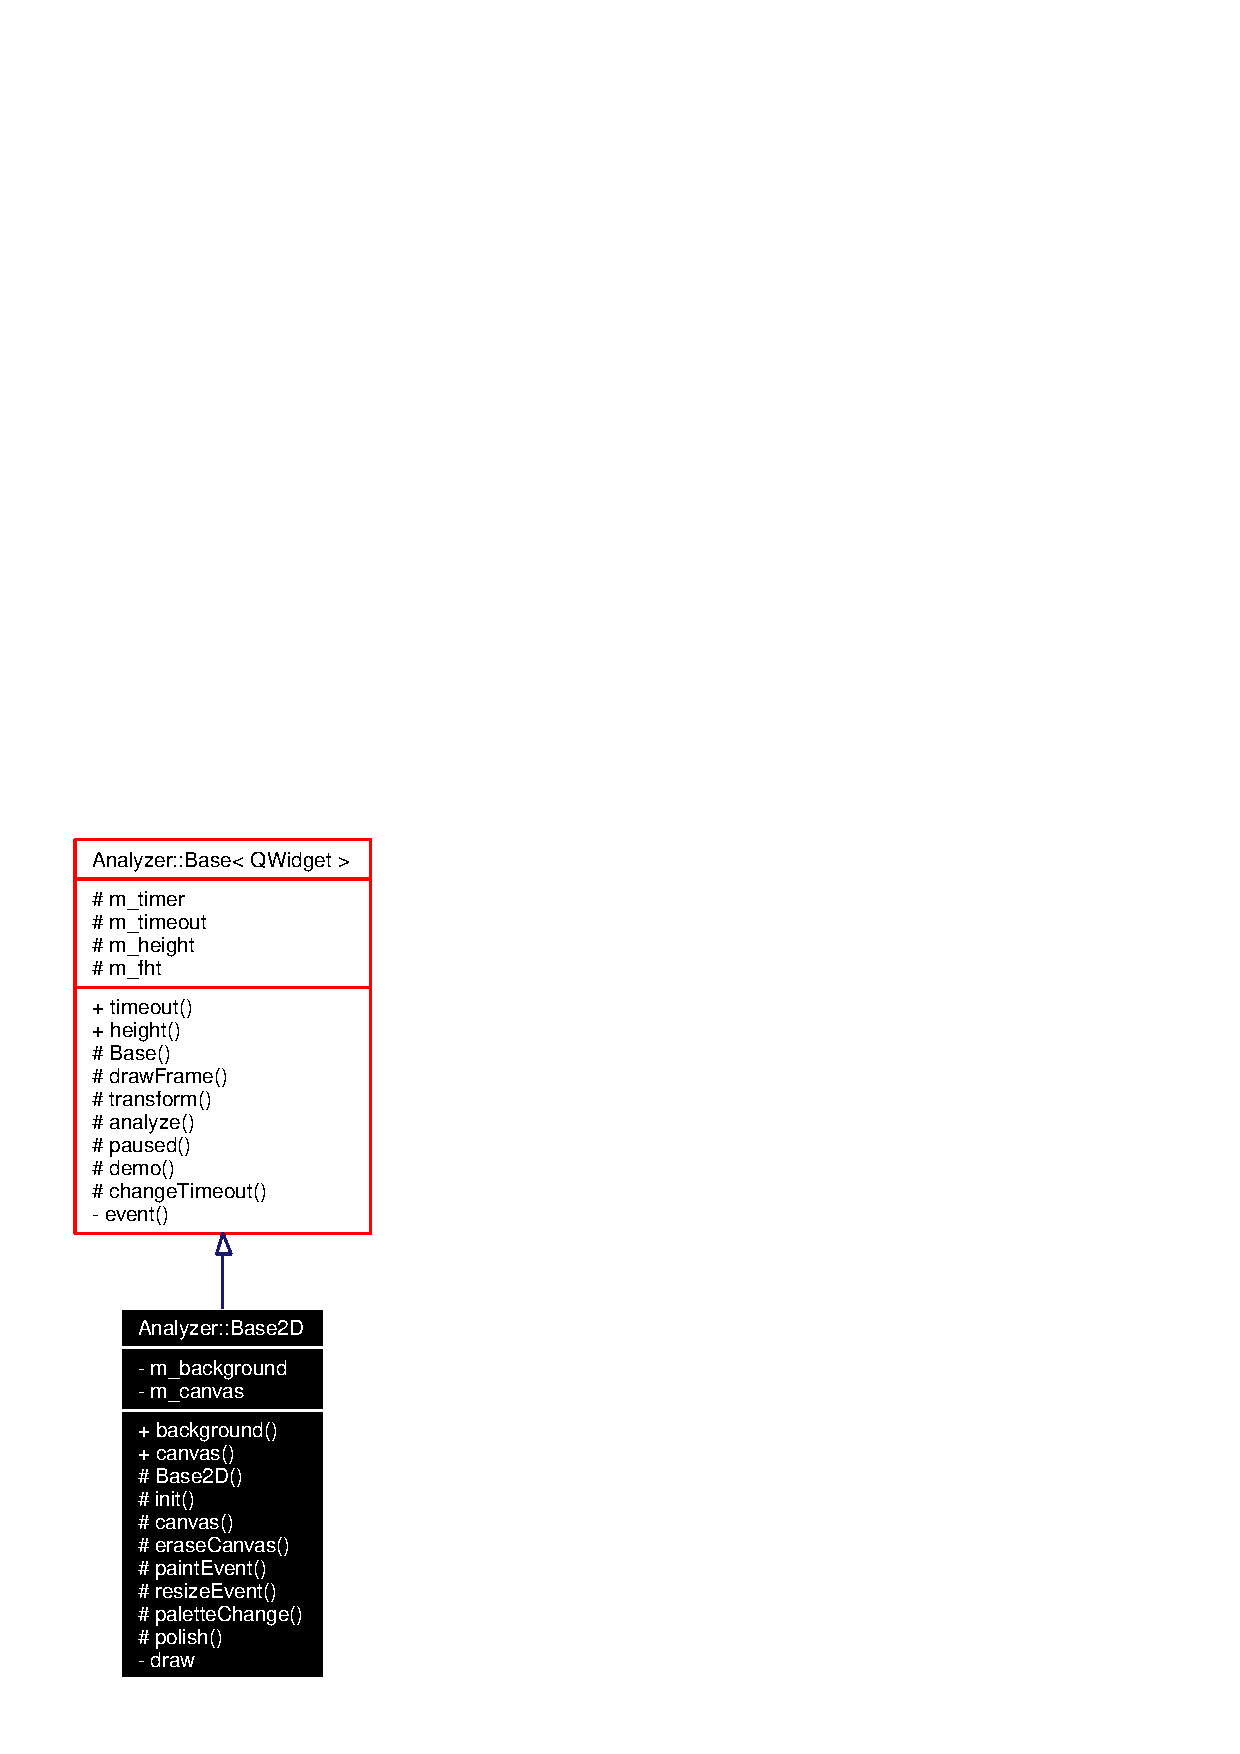
\includegraphics[width=89pt]{classAnalyzer_1_1Base2D__coll__graph}
\end{center}
\end{figure}
\subsection*{Public Member Functions}
\begin{CompactItemize}
\item 
const QPixmap $\ast$ {\bf background} () const 
\item 
const QPixmap $\ast$ {\bf canvas} () const 
\item 
uint {\bf timeout} () const
\item 
uint {\bf height} () const
\end{CompactItemize}
\subsection*{Protected Member Functions}
\begin{CompactItemize}
\item 
{\bf Base2D} ({\bf QWidget} $\ast$, uint timeout, uint scope\-Size=7)
\item 
virtual void {\bf init} ()
\item 
QPixmap $\ast$ {\bf canvas} ()
\item 
void {\bf erase\-Canvas} ()
\item 
void {\bf paint\-Event} (QPaint\-Event $\ast$)
\item 
void {\bf resize\-Event} (QResize\-Event $\ast$)
\item 
void {\bf palette\-Change} (const class QPalette \&)
\item 
void {\bf polish} ()
\item 
void {\bf draw\-Frame} ()
\item 
virtual void {\bf transform} ({\bf Scope} \&)
\item 
virtual void {\bf analyze} (const {\bf Scope} \&)=0
\item 
virtual void {\bf paused} ()
\item 
virtual void {\bf demo} ()
\item 
void {\bf change\-Timeout} (uint new\-Timeout)
\end{CompactItemize}
\subsection*{Protected Attributes}
\begin{CompactItemize}
\item 
QTimer {\bf m\_\-timer}
\item 
uint {\bf m\_\-timeout}
\item 
uint {\bf m\_\-height}
\item 
{\bf FHT} {\bf m\_\-fht}
\end{CompactItemize}
\subsection*{Private Slots}
\begin{CompactItemize}
\item 
void {\bf draw} ()
\end{CompactItemize}
\subsection*{Private Attributes}
\begin{CompactItemize}
\item 
QPixmap {\bf m\_\-background}
\item 
QPixmap {\bf m\_\-canvas}
\end{CompactItemize}


\subsection{Constructor \& Destructor Documentation}
\index{Analyzer::Base2D@{Analyzer::Base2D}!Base2D@{Base2D}}
\index{Base2D@{Base2D}!Analyzer::Base2D@{Analyzer::Base2D}}
\subsubsection{\setlength{\rightskip}{0pt plus 5cm}Analyzer::Base2D::Base2D ({\bf QWidget} $\ast$, uint {\em timeout}, uint {\em scope\-Size} = 7)\hspace{0.3cm}{\tt  [protected]}}\label{classAnalyzer_1_1Base2D_Analyzer_1_1Base2Db0}




Definition at line 150 of file analyzerbase.cpp.

References draw(), and Analyzer::Base$<$ QWidget $>$::timeout().



\footnotesize\begin{verbatim}151    : Base<QWidget>( parent, timeout, scopeSize )
152 {
153     setWFlags( Qt::WNoAutoErase ); //no flicker
154 
155     connect( &m_timer, SIGNAL( timeout() ), SLOT( draw() ) );
156 }
\end{verbatim}\normalsize 


Here is the call graph for this function:\begin{figure}[H]
\begin{center}
\leavevmode
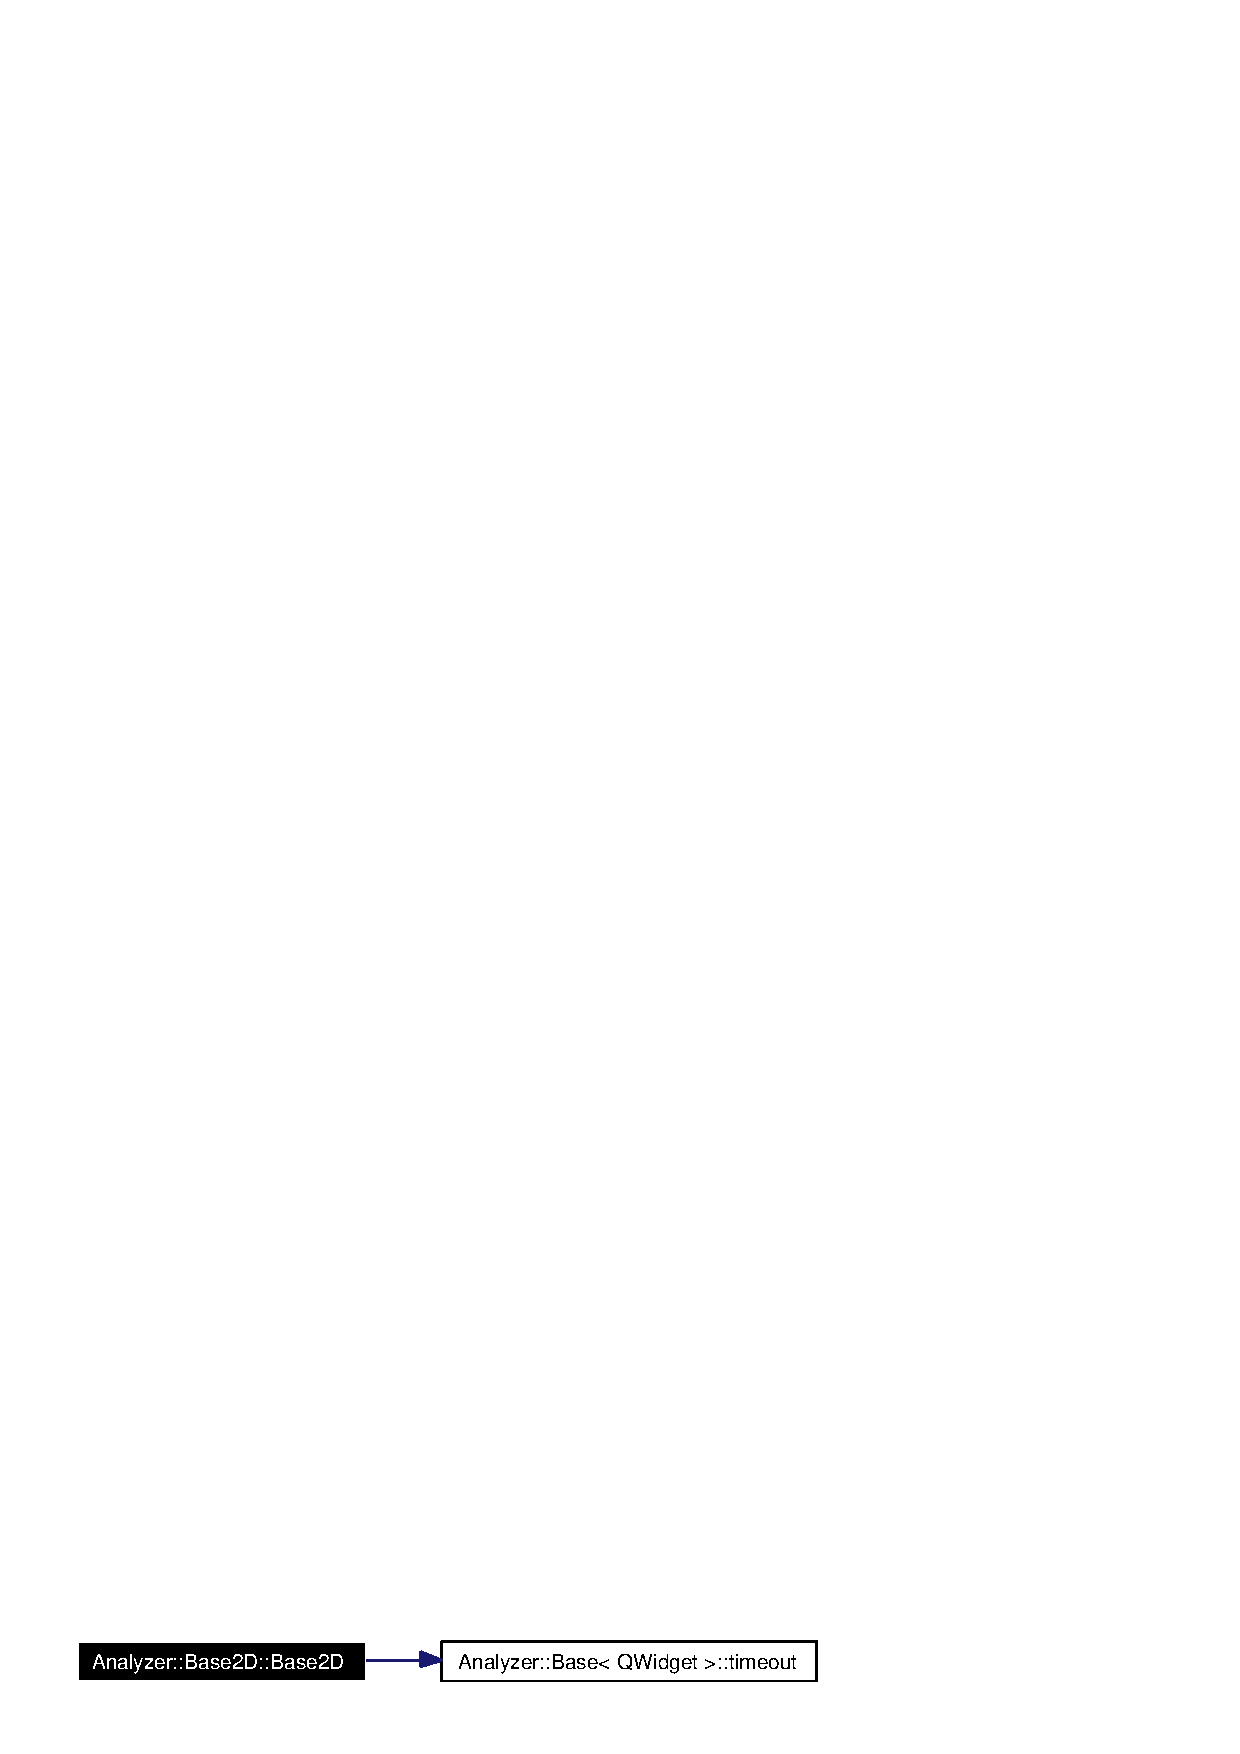
\includegraphics[width=196pt]{classAnalyzer_1_1Base2D_Analyzer_1_1Base2Db0_cgraph}
\end{center}
\end{figure}


\subsection{Member Function Documentation}
\index{Analyzer::Base2D@{Analyzer::Base2D}!analyze@{analyze}}
\index{analyze@{analyze}!Analyzer::Base2D@{Analyzer::Base2D}}
\subsubsection{\setlength{\rightskip}{0pt plus 5cm}virtual void {\bf Analyzer::Base}$<$ {\bf QWidget}  $>$::analyze (const {\bf Scope} \&)\hspace{0.3cm}{\tt  [protected, pure virtual, inherited]}}\label{classAnalyzer_1_1Base_Analyzer_1_1Baseb3}




Implemented in {\bf Sonogram} {\rm (p.\,\pageref{classSonogram_Sonograma3})}.\index{Analyzer::Base2D@{Analyzer::Base2D}!background@{background}}
\index{background@{background}!Analyzer::Base2D@{Analyzer::Base2D}}
\subsubsection{\setlength{\rightskip}{0pt plus 5cm}const QPixmap$\ast$ Analyzer::Base2D::background () const\hspace{0.3cm}{\tt  [inline]}}\label{classAnalyzer_1_1Base2D_Sonograma6}




Definition at line 75 of file analyzerbase.h.

References m\_\-background.

Referenced by erase\-Canvas().



\footnotesize\begin{verbatim}75 { return &m_background; }
\end{verbatim}\normalsize 
\index{Analyzer::Base2D@{Analyzer::Base2D}!canvas@{canvas}}
\index{canvas@{canvas}!Analyzer::Base2D@{Analyzer::Base2D}}
\subsubsection{\setlength{\rightskip}{0pt plus 5cm}QPixmap$\ast$ Analyzer::Base2D::canvas ()\hspace{0.3cm}{\tt  [inline, protected]}}\label{classAnalyzer_1_1Base2D_Sonogramb0}




Definition at line 86 of file analyzerbase.h.

References m\_\-canvas.



\footnotesize\begin{verbatim}86 { return &m_canvas; }
\end{verbatim}\normalsize 
\index{Analyzer::Base2D@{Analyzer::Base2D}!canvas@{canvas}}
\index{canvas@{canvas}!Analyzer::Base2D@{Analyzer::Base2D}}
\subsubsection{\setlength{\rightskip}{0pt plus 5cm}const QPixmap$\ast$ Analyzer::Base2D::canvas () const\hspace{0.3cm}{\tt  [inline]}}\label{classAnalyzer_1_1Base2D_Sonograma7}




Definition at line 76 of file analyzerbase.h.

References m\_\-canvas.

Referenced by Sonogram::analyze(), draw(), erase\-Canvas(), and paint\-Event().



\footnotesize\begin{verbatim}76 { return &m_canvas; }
\end{verbatim}\normalsize 
\index{Analyzer::Base2D@{Analyzer::Base2D}!changeTimeout@{changeTimeout}}
\index{changeTimeout@{changeTimeout}!Analyzer::Base2D@{Analyzer::Base2D}}
\subsubsection{\setlength{\rightskip}{0pt plus 5cm}void {\bf Analyzer::Base}$<$ {\bf QWidget}  $>$::change\-Timeout (uint {\em new\-Timeout})\hspace{0.3cm}{\tt  [inline, protected, inherited]}}\label{classAnalyzer_1_1Base_Analyzer_1_1Baseb6}




Definition at line 54 of file analyzerbase.h.



\footnotesize\begin{verbatim}55     {
56         m_timer.changeInterval( newTimeout );
57         m_timeout = newTimeout;
58     }
\end{verbatim}\normalsize 
\index{Analyzer::Base2D@{Analyzer::Base2D}!demo@{demo}}
\index{demo@{demo}!Analyzer::Base2D@{Analyzer::Base2D}}
\subsubsection{\setlength{\rightskip}{0pt plus 5cm}virtual void {\bf Analyzer::Base}$<$ {\bf QWidget}  $>$::demo ()\hspace{0.3cm}{\tt  [protected, virtual, inherited]}}\label{classAnalyzer_1_1Base_Analyzer_1_1Baseb5}




Reimplemented in {\bf Sonogram} {\rm (p.\,\pageref{classSonogram_Sonograma5})}.\index{Analyzer::Base2D@{Analyzer::Base2D}!draw@{draw}}
\index{draw@{draw}!Analyzer::Base2D@{Analyzer::Base2D}}
\subsubsection{\setlength{\rightskip}{0pt plus 5cm}void Analyzer::Base2D::draw ()\hspace{0.3cm}{\tt  [inline, private, slot]}}\label{classAnalyzer_1_1Base2D_Analyzer_1_1Base2Dk0}




Definition at line 79 of file analyzerbase.h.

References canvas(), and Analyzer::Base$<$ QWidget $>$::draw\-Frame().

Referenced by Base2D().



\footnotesize\begin{verbatim}79 { drawFrame(); bitBlt( this, 0, 0, canvas() ); }
\end{verbatim}\normalsize 
\index{Analyzer::Base2D@{Analyzer::Base2D}!drawFrame@{drawFrame}}
\index{drawFrame@{drawFrame}!Analyzer::Base2D@{Analyzer::Base2D}}
\subsubsection{\setlength{\rightskip}{0pt plus 5cm}void {\bf Analyzer::Base}$<$ {\bf QWidget}  $>$::draw\-Frame ()\hspace{0.3cm}{\tt  [protected, inherited]}}\label{classAnalyzer_1_1Base_Analyzer_1_1Baseb1}




Referenced by draw().\index{Analyzer::Base2D@{Analyzer::Base2D}!eraseCanvas@{eraseCanvas}}
\index{eraseCanvas@{eraseCanvas}!Analyzer::Base2D@{Analyzer::Base2D}}
\subsubsection{\setlength{\rightskip}{0pt plus 5cm}void Analyzer::Base2D::erase\-Canvas ()\hspace{0.3cm}{\tt  [inline, protected]}}\label{classAnalyzer_1_1Base2D_Sonogramb1}




Definition at line 87 of file analyzerbase.h.

References background(), and canvas().

Referenced by Sonogram::init(), and resize\-Event().



\footnotesize\begin{verbatim}87 { bitBlt( canvas(), 0, 0, background() ); }
\end{verbatim}\normalsize 


Here is the call graph for this function:\begin{figure}[H]
\begin{center}
\leavevmode
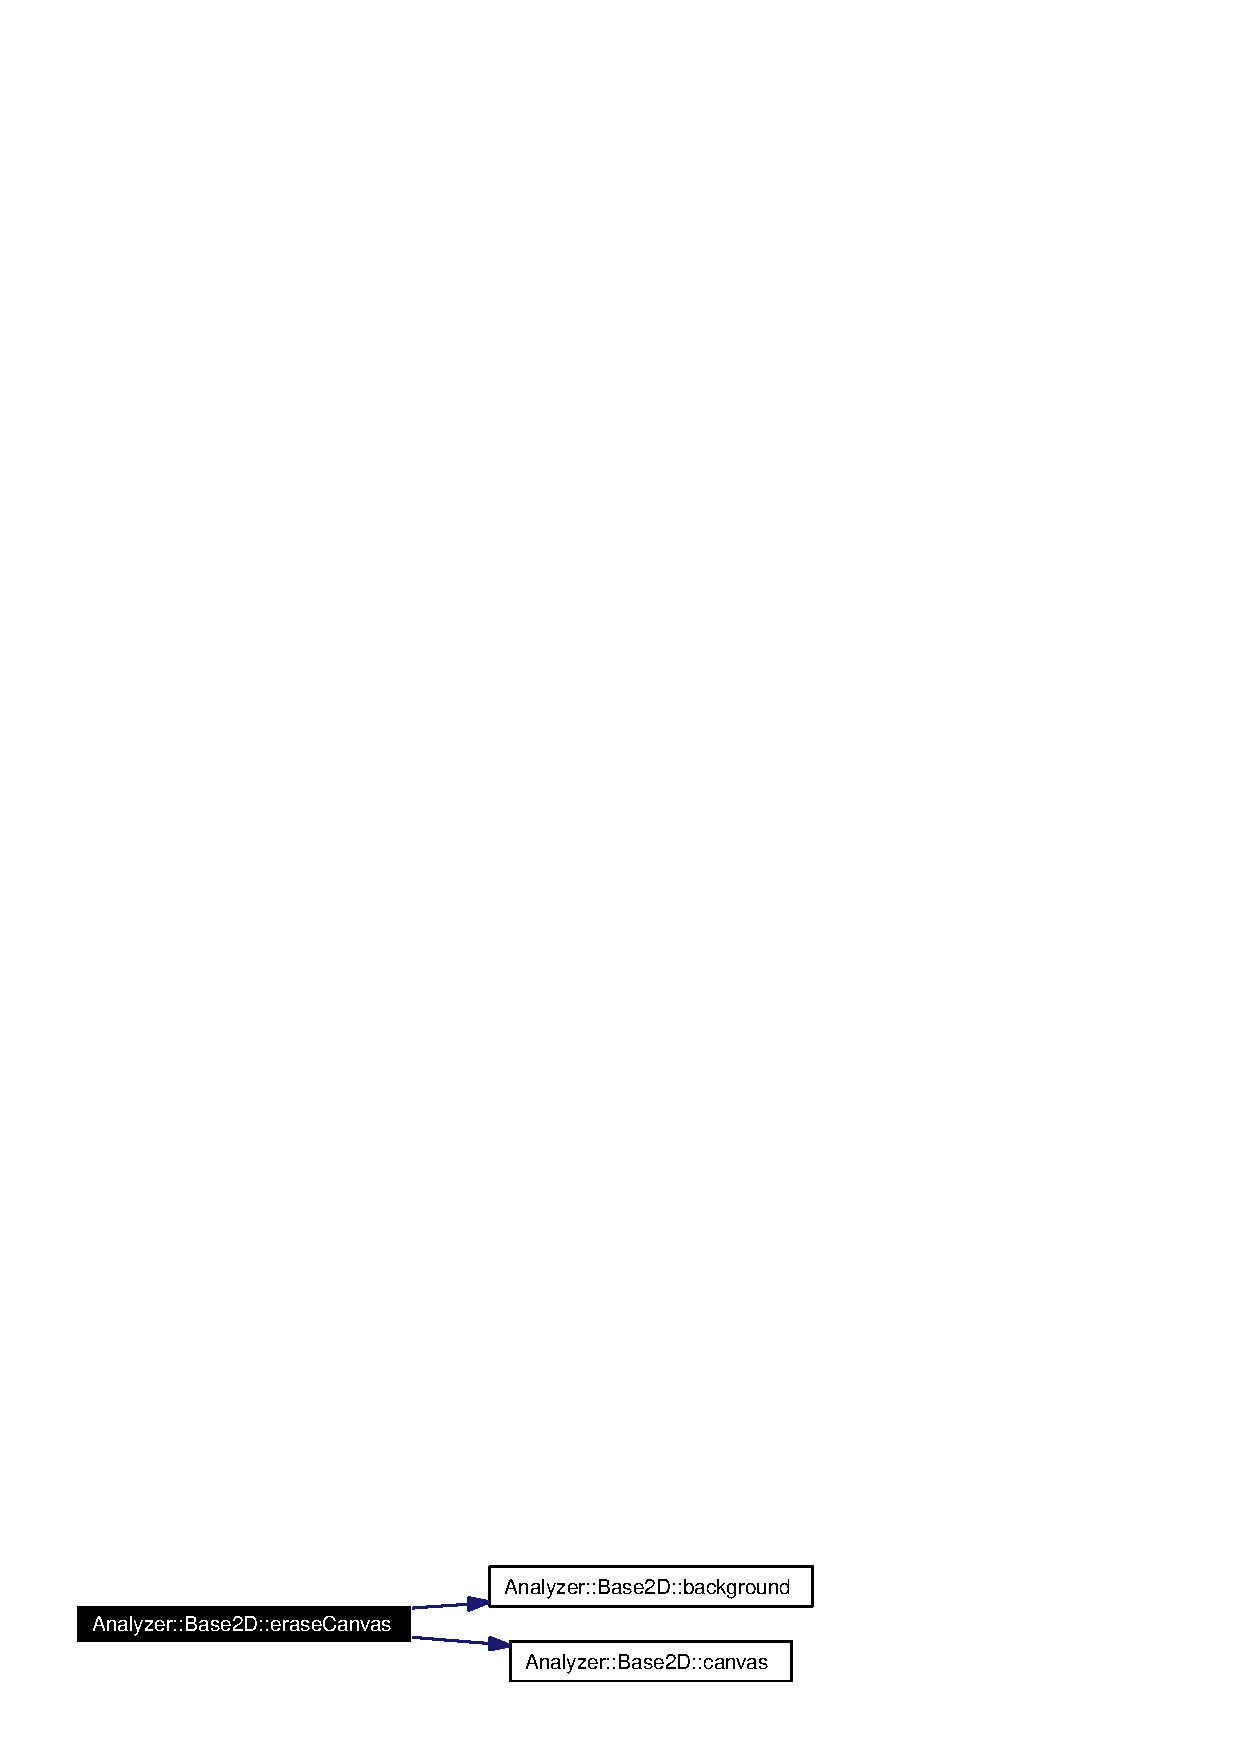
\includegraphics[width=195pt]{classAnalyzer_1_1Base2D_Sonogramb1_cgraph}
\end{center}
\end{figure}
\index{Analyzer::Base2D@{Analyzer::Base2D}!height@{height}}
\index{height@{height}!Analyzer::Base2D@{Analyzer::Base2D}}
\subsubsection{\setlength{\rightskip}{0pt plus 5cm}uint {\bf Analyzer::Base}$<$ {\bf QWidget}  $>$::height () const\hspace{0.3cm}{\tt  [inline, inherited]}}\label{classAnalyzer_1_1Base_Analyzer_1_1Basea1}




Definition at line 43 of file analyzerbase.h.

Referenced by Sonogram::analyze().



\footnotesize\begin{verbatim}43 { return m_height; }
\end{verbatim}\normalsize 
\index{Analyzer::Base2D@{Analyzer::Base2D}!init@{init}}
\index{init@{init}!Analyzer::Base2D@{Analyzer::Base2D}}
\subsubsection{\setlength{\rightskip}{0pt plus 5cm}virtual void Analyzer::Base2D::init ()\hspace{0.3cm}{\tt  [inline, protected, virtual]}}\label{classAnalyzer_1_1Base2D_Analyzer_1_1Base2Db1}




Reimplemented in {\bf Sonogram} {\rm (p.\,\pageref{classSonogram_Sonograma2})}.

Definition at line 84 of file analyzerbase.h.

Referenced by polish().



\footnotesize\begin{verbatim}84 {}
\end{verbatim}\normalsize 
\index{Analyzer::Base2D@{Analyzer::Base2D}!paintEvent@{paintEvent}}
\index{paintEvent@{paintEvent}!Analyzer::Base2D@{Analyzer::Base2D}}
\subsubsection{\setlength{\rightskip}{0pt plus 5cm}void Analyzer::Base2D::paint\-Event (QPaint\-Event $\ast$)\hspace{0.3cm}{\tt  [inline, protected]}}\label{classAnalyzer_1_1Base2D_Sonogramb2}




Definition at line 89 of file analyzerbase.h.

References canvas(), and m\_\-canvas.



\footnotesize\begin{verbatim}89 { if( !m_canvas.isNull() ) bitBlt( this, 0, 0, canvas() ); }
\end{verbatim}\normalsize 


Here is the call graph for this function:\begin{figure}[H]
\begin{center}
\leavevmode

\includegraphics[width=179pt]{classAnalyzer_1_1Base2D_Sonogramb2_cgraph}
\end{center}
\end{figure}
\index{Analyzer::Base2D@{Analyzer::Base2D}!paletteChange@{paletteChange}}
\index{paletteChange@{paletteChange}!Analyzer::Base2D@{Analyzer::Base2D}}
\subsubsection{\setlength{\rightskip}{0pt plus 5cm}void Analyzer::Base2D::palette\-Change (const class QPalette \&)\hspace{0.3cm}{\tt  [protected]}}\label{classAnalyzer_1_1Base2D_Sonogramb4}


\index{Analyzer::Base2D@{Analyzer::Base2D}!paused@{paused}}
\index{paused@{paused}!Analyzer::Base2D@{Analyzer::Base2D}}
\subsubsection{\setlength{\rightskip}{0pt plus 5cm}virtual void {\bf Analyzer::Base}$<$ {\bf QWidget}  $>$::paused ()\hspace{0.3cm}{\tt  [protected, virtual, inherited]}}\label{classAnalyzer_1_1Base_Analyzer_1_1Baseb4}


\index{Analyzer::Base2D@{Analyzer::Base2D}!polish@{polish}}
\index{polish@{polish}!Analyzer::Base2D@{Analyzer::Base2D}}
\subsubsection{\setlength{\rightskip}{0pt plus 5cm}void Analyzer::Base2D::polish ()\hspace{0.3cm}{\tt  [protected]}}\label{classAnalyzer_1_1Base2D_Sonogramb5}




Definition at line 159 of file analyzerbase.cpp.

References init().



\footnotesize\begin{verbatim}160 {
161     //TODO is there much point in this anymore?
162 
163     //we use polish for initialzing (instead of ctor)
164     //because we need to know the widget's final size
165     QWidget::polish();
166 
167     init(); //virtual
168 }
\end{verbatim}\normalsize 


Here is the call graph for this function:\begin{figure}[H]
\begin{center}
\leavevmode
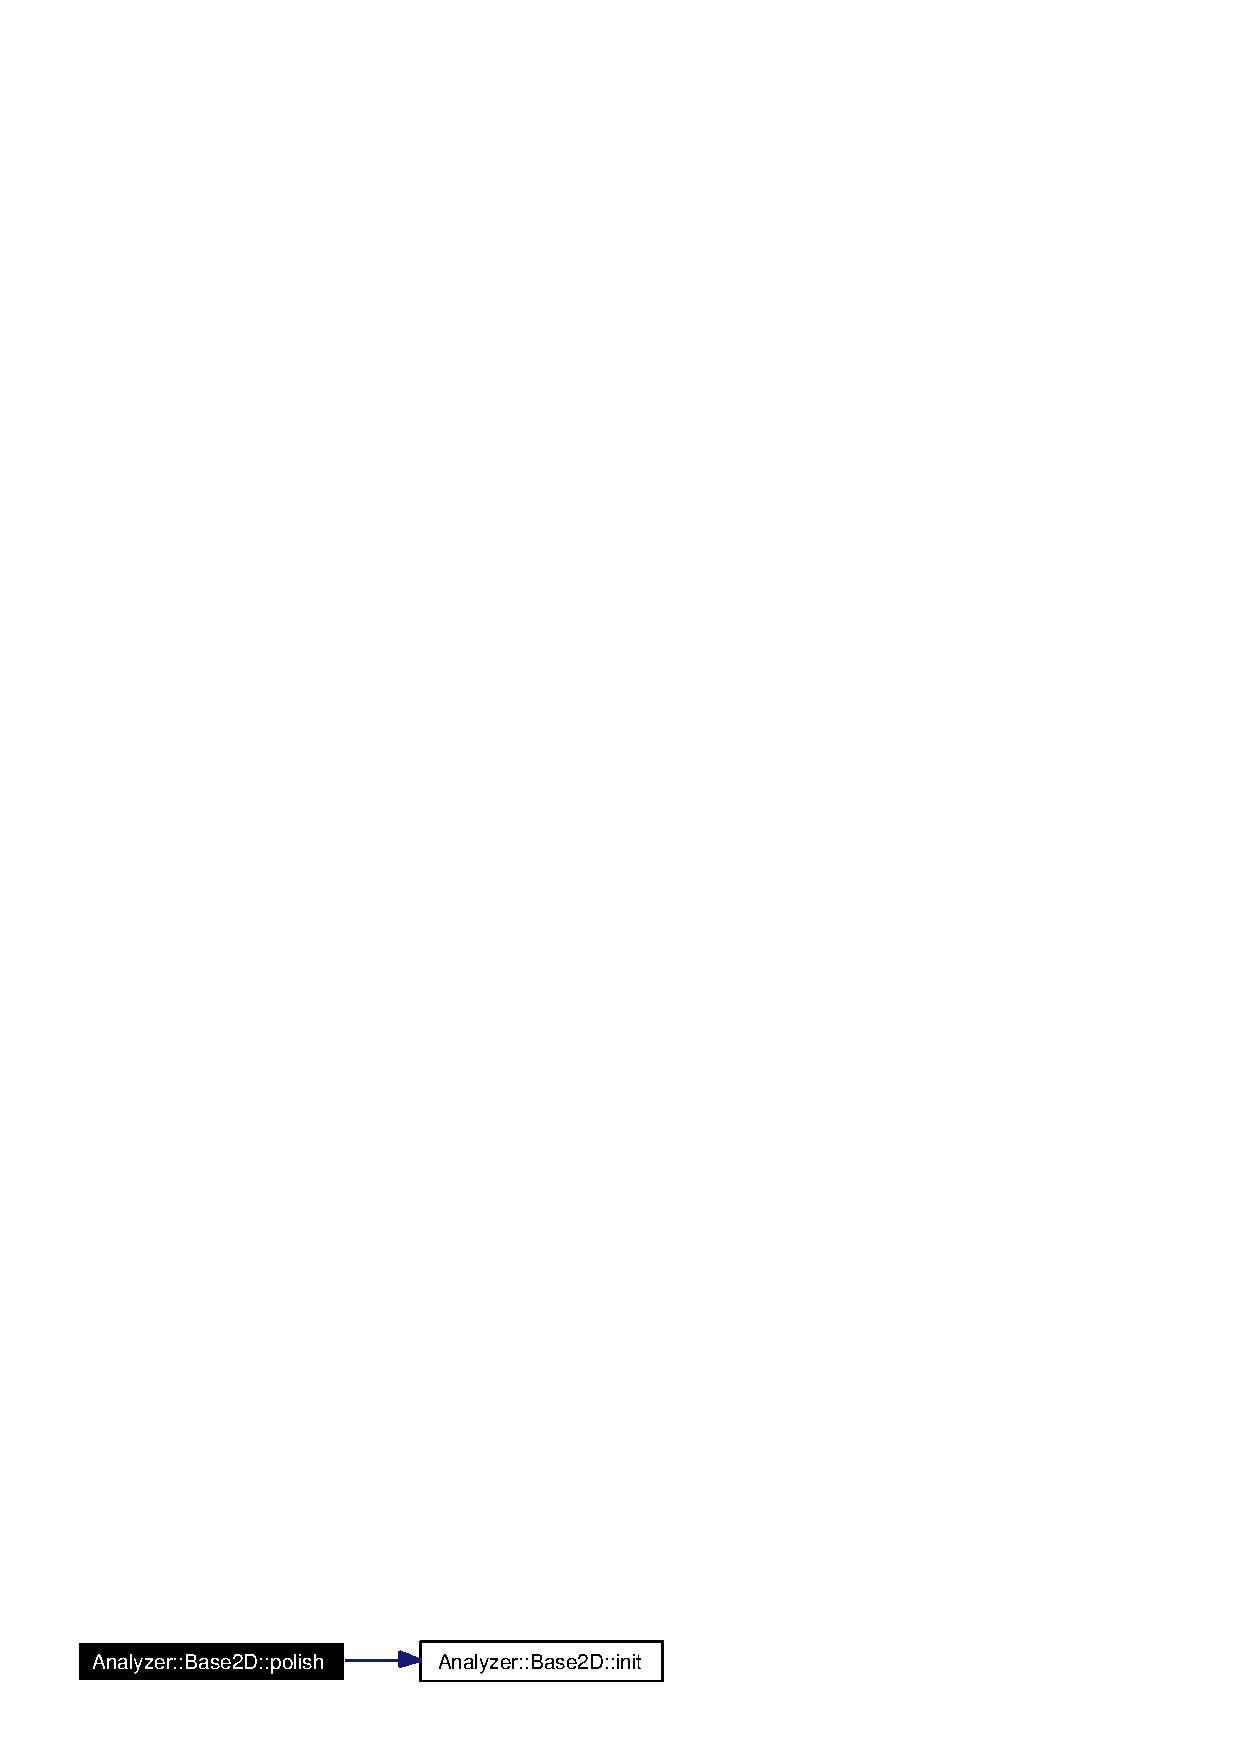
\includegraphics[width=159pt]{classAnalyzer_1_1Base2D_Sonogramb5_cgraph}
\end{center}
\end{figure}
\index{Analyzer::Base2D@{Analyzer::Base2D}!resizeEvent@{resizeEvent}}
\index{resizeEvent@{resizeEvent}!Analyzer::Base2D@{Analyzer::Base2D}}
\subsubsection{\setlength{\rightskip}{0pt plus 5cm}void Analyzer::Base2D::resize\-Event (QResize\-Event $\ast$)\hspace{0.3cm}{\tt  [protected]}}\label{classAnalyzer_1_1Base2D_Sonogramb3}




Definition at line 171 of file analyzerbase.cpp.

References erase\-Canvas(), m\_\-background, and m\_\-canvas.



\footnotesize\begin{verbatim}172 {
173     m_height = QWidget::height();
174     m_background.resize( size() );
175     m_canvas.resize( size() );
176 
177     #ifdef DRAW_GRID
178     QPainter p( &m_background );
179     p.setPen( QColor( 0x20, 0x20, 0x50 ) );
180 
181     for( uint x = 0, w = m_background.width(), h = m_background.height()-1;
182         x < w; x += 3 ) p.drawLine( x, 0, x, h );
183     for( uint y = 0, w = m_background.width()-1 , h = m_background.height();
184         y < h; y += 3 ) p.drawLine( 0, y, w, y );
185     #else
186     m_background.fill( backgroundColor() );
187     #endif
188 
189     eraseCanvas(); //this is necessary
190 
191     QWidget::resizeEvent( e );
192 }
\end{verbatim}\normalsize 


Here is the call graph for this function:\begin{figure}[H]
\begin{center}
\leavevmode
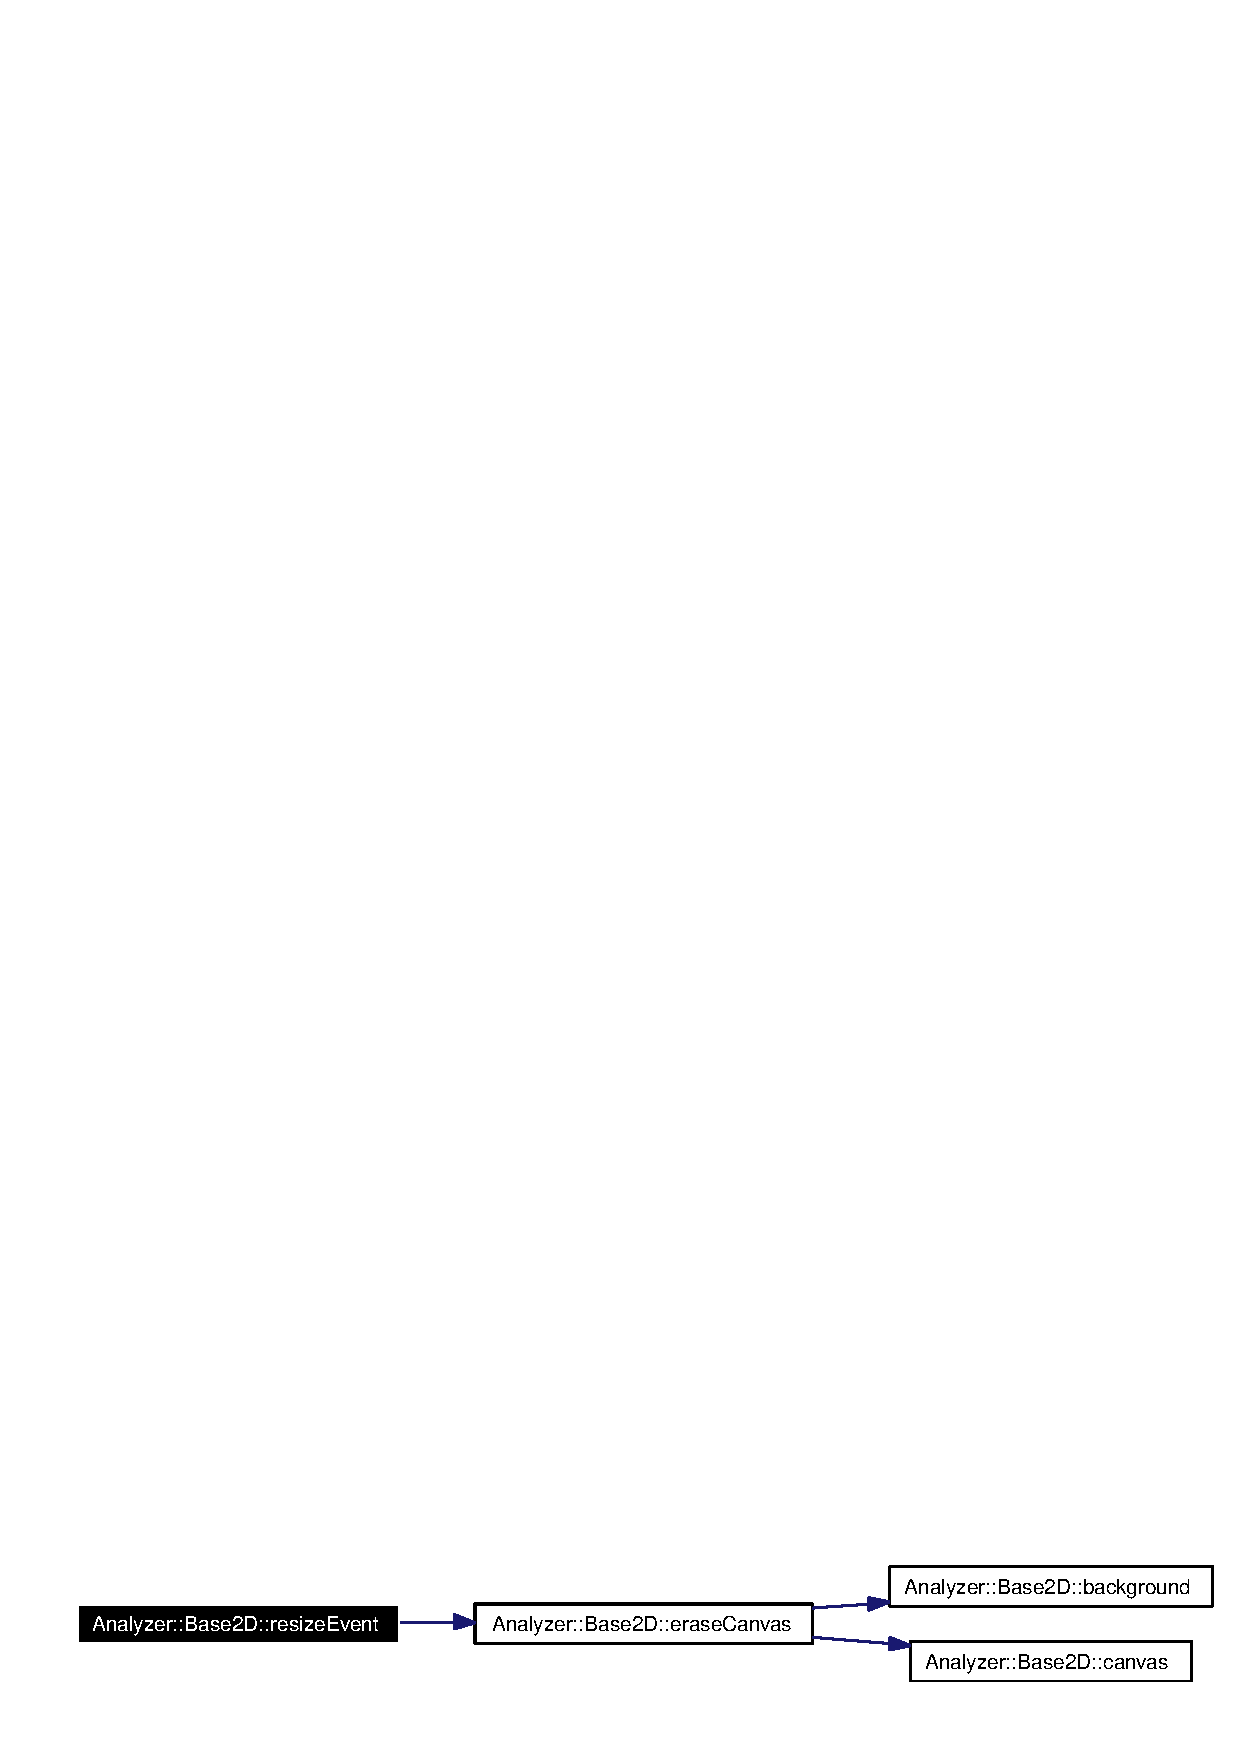
\includegraphics[width=291pt]{classAnalyzer_1_1Base2D_Sonogramb3_cgraph}
\end{center}
\end{figure}
\index{Analyzer::Base2D@{Analyzer::Base2D}!timeout@{timeout}}
\index{timeout@{timeout}!Analyzer::Base2D@{Analyzer::Base2D}}
\subsubsection{\setlength{\rightskip}{0pt plus 5cm}uint {\bf Analyzer::Base}$<$ {\bf QWidget}  $>$::timeout () const\hspace{0.3cm}{\tt  [inline, inherited]}}\label{classAnalyzer_1_1Base_Analyzer_1_1Basea0}




Definition at line 42 of file analyzerbase.h.

Referenced by Base2D().



\footnotesize\begin{verbatim}42 { return m_timeout; }
\end{verbatim}\normalsize 
\index{Analyzer::Base2D@{Analyzer::Base2D}!transform@{transform}}
\index{transform@{transform}!Analyzer::Base2D@{Analyzer::Base2D}}
\subsubsection{\setlength{\rightskip}{0pt plus 5cm}virtual void {\bf Analyzer::Base}$<$ {\bf QWidget}  $>$::transform ({\bf Scope} \&)\hspace{0.3cm}{\tt  [protected, virtual, inherited]}}\label{classAnalyzer_1_1Base_Analyzer_1_1Baseb2}




Reimplemented in {\bf Sonogram} {\rm (p.\,\pageref{classSonogram_Sonograma4})}.

\subsection{Member Data Documentation}
\index{Analyzer::Base2D@{Analyzer::Base2D}!m_background@{m\_\-background}}
\index{m_background@{m\_\-background}!Analyzer::Base2D@{Analyzer::Base2D}}
\subsubsection{\setlength{\rightskip}{0pt plus 5cm}QPixmap {\bf Analyzer::Base2D::m\_\-background}\hspace{0.3cm}{\tt  [private]}}\label{classAnalyzer_1_1Base2D_Analyzer_1_1Base2Dr0}




Definition at line 96 of file analyzerbase.h.

Referenced by background(), and resize\-Event().\index{Analyzer::Base2D@{Analyzer::Base2D}!m_canvas@{m\_\-canvas}}
\index{m_canvas@{m\_\-canvas}!Analyzer::Base2D@{Analyzer::Base2D}}
\subsubsection{\setlength{\rightskip}{0pt plus 5cm}QPixmap {\bf Analyzer::Base2D::m\_\-canvas}\hspace{0.3cm}{\tt  [private]}}\label{classAnalyzer_1_1Base2D_Analyzer_1_1Base2Dr1}




Definition at line 97 of file analyzerbase.h.

Referenced by canvas(), paint\-Event(), and resize\-Event().\index{Analyzer::Base2D@{Analyzer::Base2D}!m_fht@{m\_\-fht}}
\index{m_fht@{m\_\-fht}!Analyzer::Base2D@{Analyzer::Base2D}}
\subsubsection{\setlength{\rightskip}{0pt plus 5cm}{\bf FHT} {\bf Analyzer::Base}$<$ {\bf QWidget}  $>$::{\bf m\_\-fht}\hspace{0.3cm}{\tt  [protected, inherited]}}\label{classAnalyzer_1_1Base_Analyzer_1_1Basep3}




Definition at line 67 of file analyzerbase.h.\index{Analyzer::Base2D@{Analyzer::Base2D}!m_height@{m\_\-height}}
\index{m_height@{m\_\-height}!Analyzer::Base2D@{Analyzer::Base2D}}
\subsubsection{\setlength{\rightskip}{0pt plus 5cm}uint {\bf Analyzer::Base}$<$ {\bf QWidget}  $>$::{\bf m\_\-height}\hspace{0.3cm}{\tt  [protected, inherited]}}\label{classAnalyzer_1_1Base_Analyzer_1_1Basep2}




Definition at line 66 of file analyzerbase.h.\index{Analyzer::Base2D@{Analyzer::Base2D}!m_timeout@{m\_\-timeout}}
\index{m_timeout@{m\_\-timeout}!Analyzer::Base2D@{Analyzer::Base2D}}
\subsubsection{\setlength{\rightskip}{0pt plus 5cm}uint {\bf Analyzer::Base}$<$ {\bf QWidget}  $>$::{\bf m\_\-timeout}\hspace{0.3cm}{\tt  [protected, inherited]}}\label{classAnalyzer_1_1Base_Analyzer_1_1Basep1}




Definition at line 65 of file analyzerbase.h.\index{Analyzer::Base2D@{Analyzer::Base2D}!m_timer@{m\_\-timer}}
\index{m_timer@{m\_\-timer}!Analyzer::Base2D@{Analyzer::Base2D}}
\subsubsection{\setlength{\rightskip}{0pt plus 5cm}QTimer {\bf Analyzer::Base}$<$ {\bf QWidget}  $>$::{\bf m\_\-timer}\hspace{0.3cm}{\tt  [protected, inherited]}}\label{classAnalyzer_1_1Base_Analyzer_1_1Basep0}




Definition at line 64 of file analyzerbase.h.

The documentation for this class was generated from the following files:\begin{CompactItemize}
\item 
{\bf analyzerbase.h}\item 
{\bf analyzerbase.cpp}\end{CompactItemize}
